
%(BEGIN_QUESTION)
% Copyright 2015, Tony R. Kuphaldt, released under the Creative Commons Attribution License (v 1.0)
% This means you may do almost anything with this work of mine, so long as you give me proper credit

Work with your instructor to use the protective relay demonstration unit in the lab room to test the operation of some overcurrent relays.  Schematic wiring diagrams for this system are found in the Answer section to this question.

\vskip 10pt

(1) Configure the system to trip using the General Electric electromechanical overcurrent (ANSI code 51) relay, simulating an overcurrent condition by gently rotating the induction disk until the trip contact closes.  Examine the schematic diagram for this system and discuss what would normally cause that relay's disk to operate.

\vskip 10pt

(2) Configure the system to trip using (only) the General Electric electromechanical overcurrent (ANSI code 51) relay, and plug in a high-current load such as a large shop vacuum cleaner to generate a mild overcurrent condition.  Watch the 51 relay's induction disk slowly spin and then trip the circuit breaker open.

\vskip 10pt

(3) Configure the system to trip using (only) the SEL-501 digital overcurrent (ANSI code 50/51) relay, and plug in a high-current load such as a large shop vacuum cleaner to generate a mild overcurrent condition.  Note the time-delayed tripping action of this relay, just like the General Electric electromechanical unit.

\vskip 10pt

(4) Your instructor will decrease the pickup current value on the SEL-501 digital relay for the instantaneous overcurrent (ANSI code 50) function.  Try starting the vacuum cleaner again, and note what happens.

\vskip 10pt

(5) Your instructor will use the {\tt EVENT} command in the command-line interface for the SEL-501 digital relay to display the fault report for the last two trip events.  Analyze these reports, noting how they differ from one another.

\vskip 10pt


\underbar{file i02857}
%(END_QUESTION)





%(BEGIN_ANSWER)

\noindent
{\bf Power and CT wiring diagram:}

Note that ``C1'' and ``C2'' are two parallel-connected three-phase contactors, which act as the current-interrupting contacts for two circuit breakers.

$$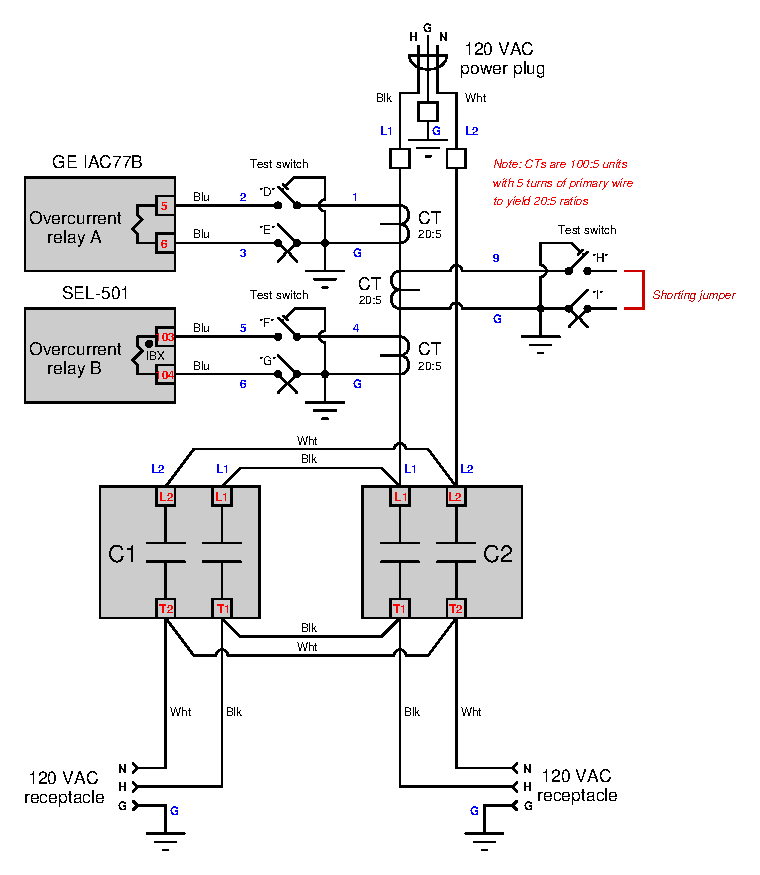
\includegraphics[width=15.5cm]{i02857x01.eps}$$

\vskip 10pt

\filbreak

\noindent
{\bf Trip circuit wiring diagram:}

Note that ``B1'' and ``B2'' are manually actuated circuit breaker units, which control the action of contactors ``C1'' and ``C2'' respectively.  Each circuit breaker has a shunt trip coil energized by one or both of the protective relays through a set of switches and ``voting diodes'' allowing either relay to control either (or both) of the two circuit breakers.

$$\includegraphics[width=15.5cm]{i02857x02.eps}$$

%(END_ANSWER)





%(BEGIN_NOTES)



%INDEX% Electric power systems: protective relays

%(END_NOTES)


